\documentclass[12pt,german]{beamer}

%\usepackage[utf8]{inputenc}
\usepackage[ngerman]{babel}
\usepackage{url}
\usepackage{graphicx}

%\usetheme{Warsaw}
\usepackage{beamerthemeshadow}


\usepackage{listings}
%\lstset{numbers=left, numberstyle=\tiny, numbersep=5pt}
\lstset{
basicstyle=\scriptsize,       % the size of the fonts that are used for the code
%numbers=left,                   % where to put the line-numbers
%numberstyle=\scriptsize,      % the size of the fonts that are used for the line-numbers
%stepnumber=5,                   % the step between two line-numbers. If it's 1 each line 
                                % will be numbered
%numbersep=5pt,                  % how far the line-numbers are from the code
showspaces=false,               % show spaces adding particular underscores
showstringspaces=false,         % underline spaces within strings
showtabs=false,                 % show tabs within strings adding particular underscores
%frame=single,	                % adds a frame around the code
tabsize=2,	                % sets default tabsize to 2 spaces
captionpos=b,                   % sets the caption-position to bottom
%breaklines=true,                % sets automatic line breaking
%breakatwhitespace=false,        % sets if automatic breaks should only happen at whitespace
%title=\lstname,                 % show the filename of files included with \lstinputlisting;
                                % also try caption instead of title
%escapeinside={\%*}{*)},         % if you want to add a comment within your code
%morekeywords={*,...}            % if you want to add more keywords to the set
}

\title{Diagrams raytracer backend}
\author{Alexander Lochmann}
\date{\today}


\begin{document}

% title page
\begin{frame}
\titlepage
\end{frame}

% table of contents
\begin{frame}
\frametitle{Inhalt}
%\setcounter{secnumdepth}{0}
\setcounter{tocdepth}{1}
\tableofcontents
\end{frame}

%%%%%%%%%%%%%%%%%%%%%%%%%%%%%%%%%%%%%%%%%%%%%%%%%%%%%%%%%%%%%%%%%%%%%%%%%%%%%%%%
\section{Einleitung}

\begin{frame}
\frametitle{Einblick}
	\begin{itemize}
		\item Raytracer in der Programmiersprache Haskell
		      als backend der DSL Diagrams
		\pause
		\item Fokus auf folgende Elemente
                \begin{itemize}
                      \item Sprachelemente benutzerfreundlich Auszuarbeiten
                      \item Schnittstelle zwischen Diagrams und Raytracer implementieren
                      \item Raytracing 
                \end{itemize}
	\end{itemize}
\end{frame}

%%%%%%%%%%%%%%%%%%%%%%%%%%%%%%%%%%%%%%%%%%%%%%%%%%%%%%%%%%%%%%%%%%%%%%%%%%%%%%%%
\section{DSL}

\begin{frame}
\frametitle{DSL Allgemein}
	\begin{itemize}
		\item Domain Specific Language
		\item spezialisiert auf eine bestimmte Domain.
		\pause
		\item 
		\item HTML ist beispielswei{\ss}e eine DSL f"ur Webseiten.
	\end{itemize}
\end{frame}

\begin{frame}
\frametitle{Beispiel Diagrams}
	\pause
	\begin{itemize}
		\item Folgendes beschreibt eine Szene in der Diagrams-DSL
		\pause
		\item sphere \# sc blue \# scale 5 \# (transform . aboutZ) (90 @@ deg) 
                      \# ambient 0.2 \# translateZ (-5) \# translateX 1 \# diffuse 0.8
                \item Diagrams Backend Schnittstelle
        \end{itemize}
\end{frame}

%%%%%%%%%%%%%%%%%%%%%%%%%%%%%%%%%%%%%%%%%%%%%%%%%%%%%%%%%%%%%%%%%%%%%%%%%%%%%%%%

\section{Raytracing}

\begin{frame}
\frametitle{Raytracing}	
  \begin{figure}
    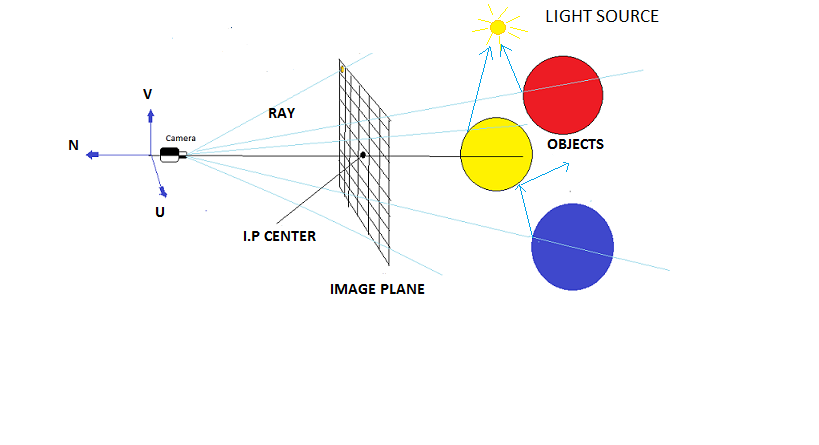
\includegraphics{ray}
    \caption{Quelle vom 11.04.2016: http://1.bp.blogspot.com/-UAPsH9kcUgM/TsWEqg2XHlI/AAAAAAAAAIg/Gq8VH5dCVnA/s1600/ImageOne.png}
  \end{figure}
\end{frame}

%%%%%%%%%%%%%%%%%%%%%%%%%%%%%%%%%%%%%%%%%%%%%%%%%%%%%%%%%%%%%%%%%%%%%%%%%%%%%%%%
\section*{}

\begin{frame}
  \begin{center}
    Danke f"ur ihre Aufmerksamkeit! \\
    Fragen?
  \end{center}
\end{frame}

\end{document}

